\documentclass[11pt]{article}
\usepackage[margin=1in]{geometry}
\usepackage{amsmath,amssymb}
\usepackage{array,booktabs}
\usepackage[table]{xcolor}
\usepackage{algorithm}
\usepackage[noend]{algpseudocode}
\usepackage{listings}
\usepackage{enumitem}
\usepackage{graphicx}
\usepackage{needspace}

\definecolor{base}{RGB}{255,243,200}   % yellow: base cases
\definecolor{path}{RGB}{210,245,220}   % green: chosen path / sources
\definecolor{ans}{RGB}{255,215,215}    % red: answer

\lstset{
  language=C++,
  basicstyle=\ttfamily\footnotesize,
  keywordstyle=\bfseries\color{blue!60!black},
  commentstyle=\color{gray},
  columns=fullflexible,
  keepspaces=true,
  frame=single,
  breaklines=true
}

\newcommand{\IfThen}[2]{\textbf{if} #1 \textbf{then} #2}

\title{Dynamic Programming Practice Set\\Questions 3, 6 and 9}
\author{Karishma Premnath}
\date{}

\begin{document}
\maketitle

%==========================================================
\section*{Question 3: Gold Mine}

\needspace{12\baselineskip}
\subsection*{T1. State, recurrence, base cases}

\noindent State: $gold[i][j]$ = max gold collected starting from cell $(i,j)$.

\medskip
\noindent Recurrence: from $(i,j)$ the miner takes $mine[i][j]$ and moves to column $j+1$ (right-up, right or right-down):
\[
gold[i][j] = mine[i][j] + \max(gold[i-1][j+1],\ gold[i][j+1],\ gold[i+1][j+1])
\]
(skip $gold[i-1][j+1]$ when $i = 0$ and $gold[i+1][j+1]$ when $i = m-1$).

\medskip
\noindent Base case: $gold[i][n-1] = mine[i][n-1]$ (last column, no more moves).

\medskip
\noindent Order: columns $n-1, n-2, \dots, 0$.

\medskip
\noindent Answer: $\max_i gold[i][0]$.

\needspace{12\baselineskip}
\subsection*{T2. Pseudocode}

\begin{algorithm}[H]
\caption{GoldMine$(mine, m, n)$}
\begin{algorithmic}[1]
\For{$i \gets 0$ \textbf{to} $m-1$}
  \State $gold[i][n-1] \gets mine[i][n-1]$
\EndFor
\For{$j \gets n-2$ \textbf{downto} $0$}
  \For{$i \gets 0$ \textbf{to} $m-1$}
    \State $best \gets gold[i][j+1]$
    \State \IfThen{$i > 0$}{$best \gets \max(best, gold[i-1][j+1])$}
    \State \IfThen{$i < m-1$}{$best \gets \max(best, gold[i+1][j+1])$}
    \State $gold[i][j] \gets mine[i][j] + best$
  \EndFor
\EndFor
\State $ans \gets gold[0][0]$
\For{$i \gets 1$ \textbf{to} $m-1$}
  \State $ans \gets \max(ans, gold[i][0])$
\EndFor
\State \Return $ans$
\end{algorithmic}
\end{algorithm}

\needspace{12\baselineskip}
\subsection*{T3. Simulation}

Mine: $\begin{bmatrix} 1 & 3 & 3\\ 2 & 1 & 4\\ 0 & 6 & 4\end{bmatrix}$.

\begin{center}
\begin{tabular}{cccl}
\toprule
Cell & $mine$ & reachable in next column & $gold$ \\
\midrule
$(0,2),(1,2),(2,2)$ & 3, 4, 4 & none (base case) & 3, 4, 4 \\
$(0,1)$ & 3 & $gold[0][2]=3,\ gold[1][2]=4$ & $3+4=7$ \\
$(1,1)$ & 1 & $3,\ 4,\ 4$ & $1+4=5$ \\
$(2,1)$ & 6 & $gold[1][2]=4,\ gold[2][2]=4$ & $6+4=10$ \\
$(0,0)$ & 1 & $gold[0][1]=7,\ gold[1][1]=5$ & $1+7=8$ \\
$(1,0)$ & 2 & $7,\ 5,\ 10$ & $2+10=12$ \\
$(2,0)$ & 0 & $gold[1][1]=5,\ gold[2][1]=10$ & $0+10=10$ \\
\bottomrule
\end{tabular}
\end{center}

\begin{center}
\begin{tabular}{c|ccc}
$gold[i][j]$ & 0 & 1 & 2 \\ \hline
0 & 8 & 7 & \cellcolor{base}3 \\
1 & \cellcolor{ans}\textbf{12} & 5 & \cellcolor{base}4 \\
2 & 10 & \cellcolor{path}10 & \cellcolor{path}4 \\
\end{tabular}
\end{center}

Yellow = base cases, red = answer $\max(8, 12, 10) = 12$, green = path $(1,0) \to (2,1) \to (2,2)$: $2 + 6 + 4 = 12$.

\needspace{12\baselineskip}
\subsection*{T4. Frequency count}

(For lines 6 and 7 the if-test is counted; it runs every time.)

\begin{center}
\begin{tabular}{clcl}
\toprule
Line & Operation & Cost & Frequency \\
\midrule
1 & for $i$ (last column) & $c_1$ & $m+1$ \\
2 & $gold[i][n-1] \gets mine[i][n-1]$ & $c_2$ & $m$ \\
3 & for $j$ (downto) & $c_3$ & $n$ \\
4 & for $i$ & $c_4$ & $(n-1)(m+1)$ \\
5 & $best \gets$ right & $c_5$ & $(n-1)m$ \\
6 & if $i>0$: right-up & $c_6$ & $(n-1)m$ \\
7 & if $i<m-1$: right-down & $c_7$ & $(n-1)m$ \\
8 & $gold[i][j] \gets mine + best$ & $c_8$ & $(n-1)m$ \\
9 & $ans \gets gold[0][0]$ & $c_9$ & 1 \\
10 & for $i$ (first column) & $c_{10}$ & $m$ \\
11 & $ans \gets \max$ & $c_{11}$ & $m-1$ \\
12 & return & $c_{12}$ & 1 \\
\bottomrule
\end{tabular}
\end{center}

\[
T(m,n) = (m+1) + m + n + (n-1)(m+1) + 4(n-1)m + 1 + m + (m-1) + 1 = \mathbf{5mn + 2n - m + 1}.
\]
For the $3\times 3$ example: $45 + 6 - 3 + 1 = 49$ line executions.

Best case = worst case = $\Theta(mn)$ (loop counts don't depend on the gold values). Memory $\Theta(mn)$.

\needspace{12\baselineskip}
\subsection*{T5. C++ with vectors}

\begin{lstlisting}
#include <iostream>
#include <vector>
#include <algorithm>
using namespace std;

int goldMine(const vector<vector<int>>& mine) {
    int m = mine.size(), n = mine[0].size();
    vector<vector<int>> gold(m, vector<int>(n, 0));
    for (int i = 0; i < m; i++) gold[i][n - 1] = mine[i][n - 1];   // last column: nowhere to go
    for (int j = n - 2; j >= 0; j--) {                             // fill from right to left
        for (int i = 0; i < m; i++) {
            int best = gold[i][j + 1];                                    // right
            if (i > 0)     best = max(best, gold[i - 1][j + 1]);          // right-up
            if (i < m - 1) best = max(best, gold[i + 1][j + 1]);          // right-down
            gold[i][j] = mine[i][j] + best;
        }
    }
    int ans = gold[0][0];
    for (int i = 1; i < m; i++) ans = max(ans, gold[i][0]);       // best starting row
    return ans;
}

int main() {
    vector<vector<int>> mine1 = {{1, 3, 3},
                                 {2, 1, 4},
                                 {0, 6, 4}};
    vector<vector<int>> mine2 = {{1, 3, 1, 5},
                                 {2, 2, 4, 1},
                                 {5, 0, 2, 3},
                                 {0, 6, 1, 2}};
    cout << "mine 1: " << goldMine(mine1) << endl;
    cout << "mine 2: " << goldMine(mine2) << endl;
    return 0;
}
\end{lstlisting}

Output:

\noindent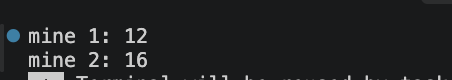
\includegraphics[width=0.6\textwidth]{out_q3.png}

\noindent Answer: 12 (path $2 \to 6 \to 4$), and 16 for the $4 \times 4$ mine. Time $\Theta(mn)$.

%==========================================================
\newpage
\section*{Question 6: Longest Palindromic Subsequence}

\needspace{12\baselineskip}
\subsection*{T1. State, recurrence, base cases}

\noindent State: $L[i][j]$ = length of the longest palindromic subsequence of $s[i..j]$.

\medskip
\noindent Recurrence:\\
if $s[i] = s[j]$: $L[i][j] = L[i+1][j-1] + 2$\\
if $s[i] \neq s[j]$: $L[i][j] = \max(L[i+1][j],\ L[i][j-1])$

\medskip
\noindent Base case: $L[i][i] = 1$, and $L[i][j] = 0$ when $i > j$ (so two equal neighbours give $0 + 2 = 2$).

\medskip
\noindent Order: by length $2, 3, \dots, n$ (diagonal by diagonal).

\medskip
\noindent Answer: $L[0][n-1]$.

\needspace{12\baselineskip}
\subsection*{T2. Pseudocode}

\begin{algorithm}[H]
\caption{LPS$(s[0..n-1])$}
\begin{algorithmic}[1]
\State create $L[0..n-1][0..n-1]$, every entry $\gets 0$
\For{$i \gets 0$ \textbf{to} $n-1$}
  \State $L[i][i] \gets 1$
\EndFor
\For{$len \gets 2$ \textbf{to} $n$}
  \For{$i \gets 0$ \textbf{to} $n - len$}
    \State $j \gets i + len - 1$
    \State \textbf{if} $s[i] = s[j]$ \textbf{then}
    \State \hspace{\algorithmicindent}$L[i][j] \gets L[i+1][j-1] + 2$
    \State \textbf{else} $L[i][j] \gets \max(L[i+1][j],\ L[i][j-1])$
  \EndFor
\EndFor
\State \Return $L[0][n-1]$
\end{algorithmic}
\end{algorithm}

\needspace{12\baselineskip}
\subsection*{T3. Simulation for $s = \text{BBABCBCAB}$}

$s[0..8] =$ B B A B C B C A B. Some cells:
\begin{itemize}[nosep]
\item $L[0][1]$: B = B, so $L[1][0] + 2 = 0 + 2 = 2$.
\item $L[1][2]$: B $\neq$ A, so $\max(L[2][2], L[1][1]) = 1$.
\item $L[4][6]$: C = C, so $L[5][5] + 2 = 3$.
\item $L[2][7]$: A = A, so $L[3][6] + 2 = 3 + 2 = 5$.
\item $L[1][7]$: B $\neq$ A, so $\max(L[2][7], L[1][6]) = \max(5, 3) = 5$.
\item $L[0][8]$: B = B, so $L[1][7] + 2 = 5 + 2 = \mathbf{7}$.
\end{itemize}

\begin{center}
\renewcommand{\arraystretch}{1.25}
\begin{tabular}{c|ccccccccc}
 & B & B & A & B & C & B & C & A & B \\ \hline
B & \cellcolor{base}1 & 2 & 2 & 3 & 3 & 5 & 5 & 5 & \cellcolor{ans}\textbf{7} \\
B &   & \cellcolor{base}1 & 1 & 3 & 3 & 3 & 3 & \cellcolor{path}5 & 7 \\
A &   &   & \cellcolor{base}1 & 1 & 1 & 3 & 3 & \cellcolor{path}5 & 5 \\
B &   &   &   & \cellcolor{base}1 & 1 & 3 & \cellcolor{path}3 & 3 & 5 \\
C &   &   &   &   & \cellcolor{base}1 & 1 & \cellcolor{path}3 & 3 & 3 \\
B &   &   &   &   &   & \cellcolor{path}1 & 1 & 1 & 3 \\
C &   &   &   &   &   &   & \cellcolor{base}1 & 1 & 1 \\
A &   &   &   &   &   &   &   & \cellcolor{base}1 & 1 \\
B &   &   &   &   &   &   &   &   & \cellcolor{base}1 \\
\end{tabular}
\end{center}

Yellow = base cases, red = $L[0][8] = 7$, green = trace back: $L[0][8]$ (B = B) $\to L[1][7]$ (B $\neq$ A, larger is $L[2][7]$) $\to L[2][7]$ (A = A) $\to L[3][6]$ (B $\neq$ C, take $L[4][6]$) $\to L[4][6]$ (C = C) $\to L[5][5]$. Palindrome: BACBCAB (BABCBAB also works).

Check: LCS(BBABCBCAB, BACBCBABB) = 7.

\needspace{12\baselineskip}
\subsection*{T4. Frequency count}

$E$ = number of cells where $s[i] = s[j]$. Line 8 runs $E$ times, line 9 runs $\frac{n(n-1)}{2} - E$ times.

\begin{center}
\begin{tabular}{clcl}
\toprule
Line & Operation & Cost & Frequency \\
\midrule
1 & create $L$, all 0 & $c_1$ & $n^2$ (entries set) \\
2 & for $i$ (diagonal) & $c_2$ & $n+1$ \\
3 & $L[i][i] \gets 1$ & $c_3$ & $n$ \\
4 & for $len$ & $c_4$ & $n$ \\
5 & for $i$ & $c_5$ & $\frac{n(n-1)}{2} + (n-1)$ \\
6 & $j \gets i + len - 1$ & $c_6$ & $\frac{n(n-1)}{2}$ \\
7 & test $s[i] = s[j]$ & $c_7$ & $\frac{n(n-1)}{2}$ \\
8 & $L \gets$ inner $+ 2$ & $c_8$ & $E$ \\
9 & $L \gets \max$ of two & $c_9$ & $\frac{n(n-1)}{2} - E$ \\
10 & return & $c_{10}$ & 1 \\
\bottomrule
\end{tabular}
\end{center}

Line 5: $\sum_{len=2}^{n}(n - len + 2) = \frac{n(n-1)}{2} + (n-1)$. Lines 8 + 9 $= \frac{n(n-1)}{2}$ for any $E$, so
\[
T(n) = n^2 + (n+1) + n + n + \Bigl[\tfrac{n(n-1)}{2} + n - 1\Bigr] + 3\cdot\tfrac{n(n-1)}{2} + 1 = \mathbf{3n^2 + 2n + 1}.
\]
$n = 9$: $243 + 18 + 1 = 262$ ($E = 12$).

Cells filled by the loop: $\frac{n(n-1)}{2} = 36$ for $n = 9$ (45 with the diagonal).

Best case = worst case = $\Theta(n^2)$ (the characters only pick line 8 or 9). Memory $\Theta(n^2)$. Brute force: $2^n$ subsequences.

\needspace{12\baselineskip}
\subsection*{T5. C++ with vectors}

\begin{lstlisting}
#include <iostream>
#include <vector>
#include <string>
#include <algorithm>
using namespace std;

int lps(const string& s) {
    int n = s.size();
    vector<vector<int>> L(n, vector<int>(n, 0));
    for (int i = 0; i < n; i++) L[i][i] = 1;                 // one character
    for (int len = 2; len <= n; len++) {                     // by substring length
        for (int i = 0; i <= n - len; i++) {
            int j = i + len - 1;
            if (s[i] == s[j])
                L[i][j] = L[i + 1][j - 1] + 2;               // use both ends (L[i+1][i] = 0 when len = 2)
            else
                L[i][j] = max(L[i + 1][j], L[i][j - 1]);     // drop one end
        }
    }
    return L[0][n - 1];
}

int main() {
    cout << "BBABCBCAB: " << lps("BBABCBCAB") << endl;
    cout << "AGBDBA: " << lps("AGBDBA") << endl;
    return 0;
}
\end{lstlisting}

Output:

\noindent
\includegraphics[width=0.6\textwidth]{out_q6.png}

\noindent Answer: 7 for BBABCBCAB (BACBCAB), 5 for AGBDBA (ABDBA). Time $\Theta(n^2)$.

%==========================================================
\newpage
\section*{Question 9: Maximum Sum Rectangle}

\needspace{12\baselineskip}
\subsection*{T1. Why fixing two columns gives the maximum subarray problem}

\noindent State: for fixed columns $l, r$: $rowSum[i] = A[i][l] + \dots + A[i][r]$.

\medskip
\noindent Reduction: a rectangle in columns $l..r$, rows $t..b$ has sum
\[
rowSum[t] + rowSum[t+1] + \dots + rowSum[b],
\]
so the best rectangle for fixed $l, r$ = max sum contiguous block of $rowSum$ = maximum subarray (Kadane).

\medskip
\noindent Kadane: $cur = \max(rowSum[i],\ cur + rowSum[i])$, $best = \max(best, cur)$.

\medskip
\noindent Base case: $cur = best = rowSum[0]$.

\medskip
\noindent Answer: max of Kadane over every pair $l \le r$.

\needspace{12\baselineskip}
\subsection*{T2. Pseudocode}

\begin{algorithm}[H]
\caption{Kadane$(a[0..m-1])$ (helper, from the lecture notes)}
\begin{algorithmic}[1]
\State $cur \gets a[0]$, $best \gets a[0]$
\For{$i \gets 1$ \textbf{to} $m-1$}
  \State $cur \gets \max(a[i],\ cur + a[i])$
  \State $best \gets \max(best, cur)$
\EndFor
\State \Return $best$
\end{algorithmic}
\end{algorithm}

\begin{algorithm}[H]
\caption{MaxRectangle$(A, m, n)$}
\begin{algorithmic}[1]
\State $best \gets -\infty$
\For{$l \gets 0$ \textbf{to} $n-1$}
  \For{$i \gets 0$ \textbf{to} $m-1$}
    \State $rowSum[i] \gets 0$
  \EndFor
  \For{$r \gets l$ \textbf{to} $n-1$}
    \For{$i \gets 0$ \textbf{to} $m-1$}
      \State $rowSum[i] \gets rowSum[i] + A[i][r]$
    \EndFor
    \State $best \gets \max(best,\ \text{Kadane}(rowSum))$
  \EndFor
\EndFor
\State \Return $best$
\end{algorithmic}
\end{algorithm}

\needspace{12\baselineskip}
\subsection*{T3. Simulation for $l = 1$, $r = 3$}

Row sums for columns 1..3: row 0: $2 - 1 - 4 = -3$; row 1: $-3 + 4 + 2 = 3$; row 2: $8 + 10 + 1 = 19$; row 3: $-1 + 1 + 7 = 7$.


\begin{center}
\begin{tabular}{lcccc}
\toprule
Row & 0 & 1 & 2 & 3 \\
\midrule
row sum for columns 1..3 & $-3$ & 3 & 19 & 7 \\
decision & start & restart ($3 > 0$) & extend ($22 > 19$) & extend ($29 > 7$) \\
Kadane: $cur$ & $-3$ & 3 & 22 & 29 \\
Kadane: $best$ & $-3$ & 3 & 22 & \textbf{29} \\
\bottomrule
\end{tabular}
\end{center}

Best block = rows 1..3, sum $3 + 19 + 7 = 29$. So the rectangle is rows 1..3, columns 1..3, sum 29 (no other $(l, r)$ does better).

\begin{center}
\renewcommand{\arraystretch}{1.25}
\begin{tabular}{c|ccccc}
 & 0 & 1 & 2 & 3 & 4 \\ \hline
0 & 1 & 2 & $-1$ & $-4$ & $-20$ \\
1 & $-8$ & \cellcolor{path}$-3$ & \cellcolor{path}4 & \cellcolor{path}2 & 1 \\
2 & 3 & \cellcolor{path}8 & \cellcolor{path}10 & \cellcolor{path}1 & 3 \\
3 & $-4$ & \cellcolor{path}$-1$ & \cellcolor{path}1 & \cellcolor{path}7 & $-6$ \\
\end{tabular}
\end{center}

Green = max rectangle, $(1,1)$ to $(3,3)$, sum 29.

\needspace{12\baselineskip}
\subsection*{T4. Frequency count}

$P = \frac{n(n+1)}{2}$ = number of pairs $l \le r$. One Kadane call on $m$ numbers $= 1 + m + (m-1) + (m-1) + 1 = 3m$ lines.

\begin{center}
\begin{tabular}{clcl}
\toprule
Line & Operation & Cost & Frequency \\
\midrule
1 & $best \gets -\infty$ & $c_1$ & 1 \\
2 & for $l$ & $c_2$ & $n+1$ \\
3 & for $i$ (reset) & $c_3$ & $n(m+1)$ \\
4 & $rowSum[i] \gets 0$ & $c_4$ & $nm$ \\
5 & for $r$ & $c_5$ & $P + n$ \\
6 & for $i$ (add column) & $c_6$ & $P(m+1)$ \\
7 & $rowSum[i] \mathrel{+}= A[i][r]$ & $c_7$ & $Pm$ \\
8 & $best \gets \max(best, \text{Kadane})$ & $c_8$ & $P$ calls, $3m$ lines each \\
9 & return & $c_9$ & 1 \\
\bottomrule
\end{tabular}
\end{center}

\begin{align*}
T(m,n) &= 1 + (n+1) + n(m+1) + nm + (P+n) + P(m+1) + Pm + P(1 + 3m) + 1\\
&= 5Pm + 3P + 2mn + 3n + 3.
\end{align*}
With $P = \frac{n(n+1)}{2}$:
\[
T(m,n) = \tfrac{5}{2}mn^2 + \tfrac{9}{2}mn + \tfrac{3}{2}n^2 + \tfrac{9}{2}n + 3 = \mathbf{\Theta(n^2 m)}.
\]
$4 \times 5$ example ($P = 15$): $300 + 45 + 40 + 15 + 3 = 403$.

Best case = worst case = $\Theta(n^2 m)$ (values in $A$ don't change the counts). Memory $\Theta(m)$ for $rowSum$.

Brute force: $\frac{m(m+1)}{2}\cdot\frac{n(n+1)}{2}$ rectangles (150 here), each summed in up to $mn$ steps $\Rightarrow \Theta(m^3 n^3)$; $\Theta(m^2 n^2)$ with 2D prefix sums. Kadane removes the choice of $t, b$ $\Rightarrow \Theta(n^2 m)$.

\needspace{12\baselineskip}
\subsection*{T5. C++ with vectors}

\begin{lstlisting}
#include <iostream>
#include <vector>
#include <climits>
using namespace std;

// Kadane on a[0..m-1]; also reports where the best block starts and ends
int kadane(const vector<int>& a, int& top, int& bottom) {
    int cur = a[0], best = a[0], start = 0;
    top = bottom = 0;
    for (int i = 1; i < (int)a.size(); i++) {
        if (a[i] > cur + a[i]) { cur = a[i]; start = i; }   // restart at i
        else cur = cur + a[i];                              // extend
        if (cur > best) { best = cur; top = start; bottom = i; }
    }
    return best;
}

int main() {
    vector<vector<int>> A = {{ 1,  2, -1, -4, -20},
                             {-8, -3,  4,  2,   1},
                             { 3,  8, 10,  1,   3},
                             {-4, -1,  1,  7,  -6}};
    int m = A.size(), n = A[0].size();
    int best = INT_MIN, bl = 0, br = 0, bt = 0, bb = 0;
    for (int l = 0; l < n; l++) {
        vector<int> rowSum(m, 0);
        for (int r = l; r < n; r++) {
            for (int i = 0; i < m; i++) rowSum[i] += A[i][r];   // add column r only
            int top, bottom;
            int s = kadane(rowSum, top, bottom);
            if (s > best) { best = s; bl = l; br = r; bt = top; bb = bottom; }
        }
    }
    cout << "max sum: " << best << endl;
    cout << "top-left (" << bt << ", " << bl << "), bottom-right (" << bb << ", " << br << ")" << endl;
    return 0;
}
\end{lstlisting}

Output:

\noindent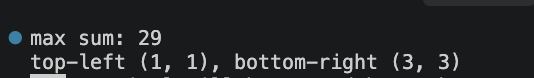
\includegraphics[width=0.6\textwidth]{out_q9.png}

\noindent Answer: rows 1..3, columns 1..3, sum 29. Time $\Theta(n^2 m)$.

%==========================================================
\section*{Summary rows to fill in}

\begin{center}
\begin{tabular}{cp{2.6cm}p{1.8cm}p{6.2cm}c}
\toprule
\# & Problem & State & Recurrence & Time \\
\midrule
3 & Gold mine & $gold[i][j]$ & $mine[i][j] + \max(\text{3 cells in column } j+1)$ & $\Theta(mn)$ \\
6 & LPS & $L[i][j]$ & match: $L[i+1][j-1]+2$, else $\max(L[i+1][j], L[i][j-1])$ & $\Theta(n^2)$ \\
9 & Max sum rectangle & $rowSum$, $cur$ & every $l \le r$: Kadane on row sums & $\Theta(n^2 m)$ \\
\bottomrule
\end{tabular}
\end{center}



\end{document}
